\section{X-Learning organization}
\label{sec:x-learning_organization}

  Durante la fase iniziale di analisi e progettazione si è evidenziata la necessità di suddividere il lavoro in due macro-blocchi public e admin. L’idea base è stata quella di delegare tutti compiti di creazione, gestione al lato admin e delegare invece la gestione della fruizione dei contenuti al lato client.
Inoltre questa scelta è dettata dalla volontà di rendere indipendenti tra di loro i vari componenti per permettere una maggiore flessibilità e garantire anche maggiore sicurezza posizionando per esempio il client in un server diverso da quello admin.
Il risultato finale ottenuto è quello di due piattaforme totalmente indipendenti che possono coesistere tra loro, permettendo massima autonomia e garantendo un elevato indice di coesione.


\begin{figure}[htbp] %  figure placement: here, top, bottom
 \centering
 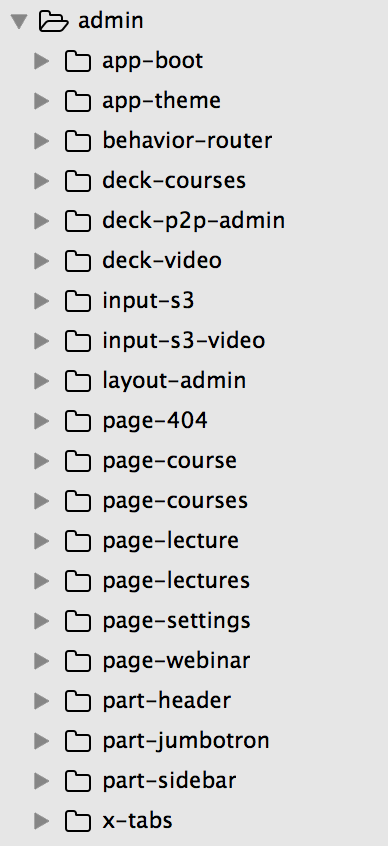
\includegraphics[width=0.5\linewidth]{images/chapter3/admin.png}\hfill
 \caption[admin hierarchy]{Admin hierarchy}
 \label{fig:fourV}
\end{figure}

\begin{figure}[htbp] %  figure placement: here, top, bottom
 \centering
 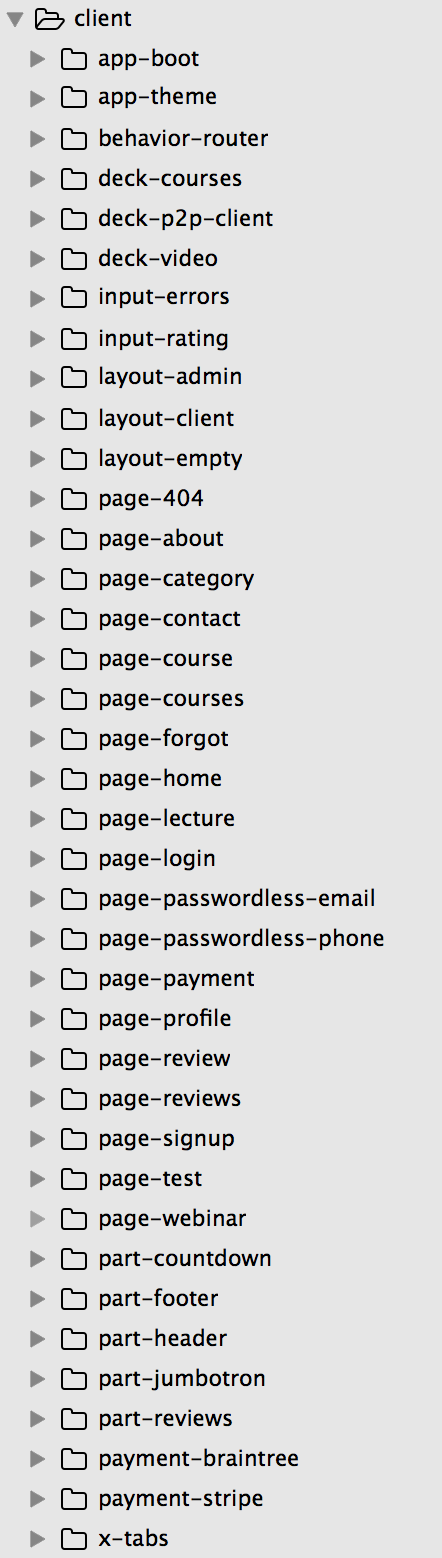
\includegraphics[width=0.5\linewidth]{images/chapter3/client.png}\hfill
 \caption[Client hierarchy]{Client hierarchy}
 \label{fig:fourV}
\end{figure}

\newpage